%杨舒云的实验报告编辑界面,使用了Huanyu Shi,2019级的模板,杨舒云在此拜谢ORZ!

%!TEX program = xelatex
\documentclass[dvipsnames, svgnames,a4paper,11pt]{article}
% ----------------------------------------------------- 
%	加边框的命令
%	参考:https://tex.stackexchange.com/questions/531559/how-to-add-the-page-border-for-first-two-pages-in-latex
\usepackage{tikz}
\usetikzlibrary{calc}
\usepackage{eso-pic}
\AddToShipoutPictureBG{%
\begin{tikzpicture}[overlay,remember picture]
\draw[line width=0.6pt] % 边框粗细
    ($ (current page.north west) + (0.6cm,-0.6cm) $)
    rectangle
    ($ (current page.south east) + (-0.6cm,0.6cm) $); % 边框位置
\end{tikzpicture}}


\usepackage{xcolor}
\definecolor{c1}{HTML}{086173} % 目录颜色 原版为2752C9 紫灰色535AAA 蓝紫色0B0DB7 深蓝色070F94 湖绿色219394 松石灰绿086173
\definecolor{c2}{HTML}{E20129} % 引用颜色 原版\definecolor{c2}{RGB}{190,20,83} 橙色F24729

\usepackage{ctex}
\usepackage[top=28mm,bottom=28mm,left=15mm,right=15mm]{geometry}
\usepackage{hyperref} 
\hypersetup{
	colorlinks,
	linktoc = section, % 超链接位置,选项有section, page, all
	linkcolor = c1, % linkcolor 目录颜色
	citecolor = c1  % citecolor 引用颜色
}
\usepackage{amsmath,enumerate,multirow,float}
\usepackage{tabularx}
\usepackage{tabu}
\usepackage{subfig}
\usepackage{fancyhdr}
\usepackage{graphicx}
\usepackage{wrapfig}  
\usepackage{physics}
\usepackage{appendix}
\usepackage{amsfonts}

%
\usepackage{tcolorbox}
\tcbuselibrary{skins,breakable}
\newtcolorbox{tbox}[2][]{
    colframe=black!70!,
    breakable,
    enhanced,
	boxrule =0.5pt,
    title = {#2},
    fonttitle = \large\kaishu\bfseries,
	drop fuzzy shadow,
    #1
}
\newtcolorbox[auto counter,number within=section]{question}[1][]{
  top=2pt,bottom=2pt,arc=1mm,
  boxrule=0.5pt,
%   frame hidden,
  breakable,
  enhanced, %跨页后不会显示下边框
  coltitle=c1!80!gray,
  colframe=c1,
  colback=c1!3!white,
  drop fuzzy shadow,
  title={思考题~\thetcbcounter:\quad},
  fonttitle=\bfseries,
  attach title to upper,
  #1
}

% ---------------------------------------------------------------------
%	利用cleveref改变引用格式,\cref是引用命令
\usepackage{cleveref}
\crefformat{figure}{#2{\textcolor{c2}{Figure #1}}#3} % 图片的引用格式
\crefformat{equation}{#2{(\textcolor{c2}{#1})}#3} % 公式的引用格式
\crefformat{table}{#2{\textcolor{c2}{Table #1}}#3} % 表格的引用格式


% ---------------------------------------------------------------------
%	页眉页脚设置
\fancypagestyle{plain}{\pagestyle{fancy}}
\pagestyle{fancy}
\lhead{\kaishu 中山大学物理与天文学院电子技术实验\uppercase\expandafter{\romannumeral1}} % 左边页眉,学院 + 课程
\rhead{\kaishu 实验报告By杨舒云\&戴鹏辉} % 右边页眉,实验报告标题
\cfoot{\thepage} % 页脚,中间添加页码


% ---------------------------------------------------------------------
%	对目录、章节标题的设置
\renewcommand{\contentsname}{\centerline{\huge 目录}}
\usepackage{titlesec}
\usepackage{titletoc}
% \titleformat{章节}[形状]{格式}{标题序号}{序号与标题间距}{标题前命令}[标题后命令]
\titleformat{\section}{\centering\LARGE\songti}{}{1em}{}

% ---------------------------------------------------------------------
%   listing代码环境设置
\usepackage{listings}
\lstloadlanguages{python}
\lstdefinestyle{pythonstyle}{
backgroundcolor=\color{gray!5},
language=python,
frameround=tftt,
frame=shadowbox, 
keepspaces=true,
breaklines,
columns=spaceflexible,                   
basicstyle=\ttfamily\small, % 基本文本设置,字体为teletype,大小为scriptsize
keywordstyle=[1]\color{c1}\bfseries, 
keywordstyle=[2]\color{Red!70!black},   
stringstyle=\color{Purple},       
showstringspaces=false,
commentstyle=\ttfamily\scriptsize\color{green!40!black},%注释文本设置,字体为sf,大小为smaller
tabsize=2,
morekeywords={as},
morekeywords=[2]{np, plt, sp},
numbers=left, % 代码行数
numberstyle=\it\tiny\color{gray}, % 代码行数的数字字体设置
stepnumber=1,
rulesepcolor=\color{gray!30!white}
}




% ---------------------------------------------------------------------
%	其他设置
\def\degree{${}^{\circ}$} % 角度
\graphicspath{{./images/}} % 插入图片的相对路径
\allowdisplaybreaks[4]  %允许公式跨页 
\usepackage{lipsum}
\usepackage{adjustbox}
%\usepackage{mathrsfs} % 字体
\captionsetup[figure]{name=Figure} % 图片形式
\captionsetup[table]{name=Table} % 表格形式

\begin{document}
	
	
	
	% 实验报告封面	
	
	% 顶栏
	\begin{table}
		\renewcommand\arraystretch{1.7}
		\begin{tabularx}{\textwidth}{
				|X|X|X|X
				|X|X|X|X|}
			\hline
			\multicolumn{2}{|c|}{预习报告}&\multicolumn{2}{|c|}{实验记录}&\multicolumn{2}{|c|}{分析讨论}&\multicolumn{2}{|c|}{总成绩}\\
			\hline
			\LARGE25 & & \LARGE25 & & \LARGE30 & & \LARGE80 & \\
			\hline
		\end{tabularx}
	\end{table}
	% ---
	
	% 信息栏
	\begin{table}
		\renewcommand\arraystretch{1.7}
		\begin{tabularx}{\textwidth}{|X|X|X|X|}
			\hline
			年级、专业: & 2022级 物理学 &组号: & 实验组E2\\
			\hline
			姓名: & 戴鹏辉、杨舒云  & 学号: & 22344016、223444020\\
			\hline
			实验时间: & 2024/03/04 & 教师签名: & \\
			\hline
		\end{tabularx}
	\end{table}
	% ---
	
	% 大标题
	\begin{center}
		\LARGE ET1-3 \quad 基尔霍夫定律和叠加原理
	\end{center}
	% ---
	
	% 注意事项
	
	% 基本
	\textbf{【实验报告注意事项】}
	\begin{enumerate}
		\item 实验报告由三部分组成:
		\begin{enumerate}
			\item 预习报告:课前认真研读实验讲义,弄清实验原理;实验所需的仪器设备、用具及其使用、完成课前预习思考题;了解实验需要测量的物理量,并根据要求提前准备实验记录表格(可以参考实验报告模板,可以打印)。\textcolor{red}{\textbf{(20分)}}
			\item 实验记录:认真、客观记录实验条件、实验过程中的现象以及数据。实验记录请用珠笔或者钢笔书写并签名(\textcolor{red}{\textbf{用铅笔记录的被认为无效}})。\textcolor{red}{\textbf{保持原始记录,包括写错删除部分,如因误记需要修改记录,必须按规范修改。}}(不得输入电脑打印,但可扫描手记后打印扫描件);离开前请实验教师检查记录并签名。\textcolor{red}{\textbf{(30分)}}
			\item 数据处理及分析讨论:处理实验原始数据(学习仪器使用类型的实验除外),对数据的可靠性和合理性进行分析;按规范呈现数据和结果(图、表),包括数据、图表按顺序编号及其引用;分析物理现象(含回答实验思考题,写出问题思考过程,必要时按规范引用数据);最后得出结论。\textcolor{red}{\textbf{(30分)}}
		\end{enumerate}
		\textbf{实验报告就是将预习报告、实验记录、和数据处理与分析合起来,加上本页封面。\textcolor{red}{(80分)}}
		\item 每次完成实验后的一周内交\textbf{实验报告}(特殊情况不能超过两周)。
		\item \textbf{其它注意事项}:
		\begin{enumerate}
			\item 请认真查看并理解实验讲义第一章内容;
			\item 注意实验器材的合理使用;
			\item 使用结束使用各种仪器之后需要将其放回原位。
		\end{enumerate}
	\end{enumerate}
	
	% 安全
	%	\textbf{【实验安全注意事项】}	
	%	\begin{enumerate}
		%		\item 
		%	\end{enumerate}
	
	% ---
	
	% 特别鸣谢
	\textbf{【特别鸣谢及模板说明】}	
	
	感谢2019级学长石寰宇为本实验报告提供\LaTeX 模板。\textcolor{red}{\textbf{由于原实验报告模板缺少实验编号,为方便在电脑上整理,故添加自命名编号}}
	% ---
	
	
	
	% 目录
	\clearpage
	\tableofcontents
	\clearpage
	% ---
	
	
	
	% 预习报告	
	
	% 小标题
	\setcounter{section}{0}
	\section{ET1-3 基尔霍夫定律和叠加原理 \quad\heiti 预习报告}
	% ---
	
	% 实验目的
	\subsection{实验目的}
	\begin{enumerate}
		\item 加深对基尔霍夫定律的理解。 
		\item 学习验证定律的方法和仪器仪表的正确使用。 
		\item 研究叠加原理的成立条件并在线性电路中验证叠加原理。
	\end{enumerate}
	% ---
	
	% 仪器用具
	\subsection{仪器用具}
	\begin{table}[htbp]
		\centering
		\renewcommand\arraystretch{1.6}
		% \setlength{\tabcolsep}{10mm}
		\begin{tabular}{|p{0.05\textwidth}|p{0.20\textwidth}|p{0.05\textwidth}|p{0.5\textwidth}|}
			\hline
			编号& 仪器用具名称 & 数量 &  主要参数(型号,测量范围,测量精度等)及备注 \\
			\hline
			1& 电路原理箱或板 & 1 &  \\
			\hline
			2& 稳压源 & 1 &  \\
			\hline
			3& 直流电流源 & 1 &  \\
			\hline
			4& 直流电流表 & 3 &  \\
			\hline
			5& 直流电压表 & 2 &  \\
			\hline
			6& 电流表专用线 & 3 &  \\
			\hline
			7& 2号实验导线 & n &  \\
			\hline
			8& 其它 & -- &  \\
			\hline
		\end{tabular}
	\end{table}
	% ---
	
	% 原理概述
	\subsection{原理概述}
	\begin{enumerate}
		\item \textbf{基尔霍夫定律:}
		
		基尔霍夫定律是电路分析中的两个基本定律,分别是基尔霍夫电流定律(KCL)和基尔霍夫电压定律(KVL)。
		
		\begin{itemize}
			\item \textbf{基尔霍夫电流定律(KCL):} 该定律规定了在任何电路中,流入某节点的电流总和等于流出该节点的电流总和。简而言之,电路中的电流守恒。数学表达式为:$\sum I_{\text{in}} = \sum I_{\text{out}}$
			
			\item \textbf{基尔霍夫电压定律(KVL):} 该定律规定了沿着任意闭合电路路径的电压总和等于零。简而言之,电路中的电压守恒。数学表达式为:$\sum V = 0$
		\end{itemize}
		
		这两个定律是电路分析的基石,通过它们可以简化复杂电路的分析过程。
		
		\item \textbf{线性系统的叠加原理:}
		
		线性系统的叠加原理是指如果一个系统是线性的,则它的响应可以通过分别计算各个输入信号产生的响应,然后将这些响应相加而得到。在电路理论中,这个原理可以用于分析具有多个输入信号的线性电路。
		
		具体而言,对于一个线性电路,如果施加多个输入信号,则每个输入信号单独作用时产生的响应可以被分别计算。而当这些输入信号同时作用时,系统的总响应等于各个输入信号单独作用时的响应的代数和。
		
	\end{enumerate}
	% ---
	
	\subsection{电路设计与仿真}
	\begin{enumerate}
		\item \textbf{电路设计}
		
		基于实验原理,为了探究KCL、KVL和叠加原理,我们进行了理论计算并设计了四个实验电路。接下来对四个电路图逐个作说明。
		
		\begin{enumerate}
			\item 电路一(如图所示)
			
			\begin{figure}[htbp]
				\centering
				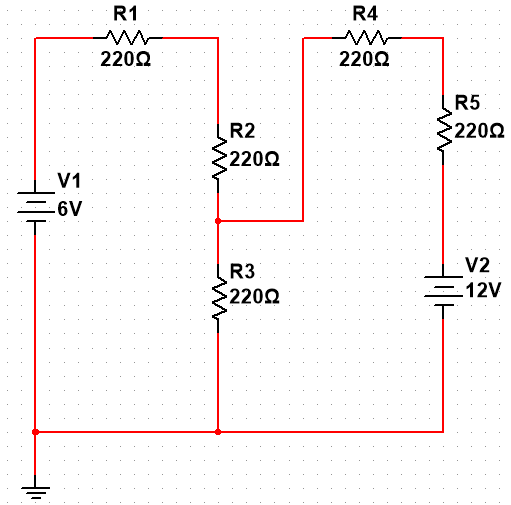
\includegraphics[width=0.4\textwidth]{ET1_3_A1-1.png}
				\caption{电路一}
				\label{fig:fig1-1}
			\end{figure}
			
			\begin{enumerate}
				\item 电路描述
				
				\begin{itemize}
					\item 电源:有两个电源,$V1$ 是 $6$ 伏特,$V2$ 是 $12$ 伏特。
					\item 电阻:有五个标有相同阻值($220$ 欧姆)的电阻,分别标为 $R1$, $R2$, $R3$, $R4$, 和 $R5$。
				\end{itemize}
				
				\item 电路连接
				
				\begin{itemize}
					\item $R1$ 与 $V1$ 串联连接,构成了电路的左侧部分。
					\item $R4$ 与 $V2$ 串联连接,构成了电路的右侧部分。
					\item $R2$ 的一端与 $R1$ 和 $V1$ 的连接点相连,另一端则与 $R3$ 和 $R4$ 的连接点相连。
					\item $R3$ 的另一端则直接与负极相连,形成了一个分支。
					\item $R5$ 直接跨接在 $V2$ 的两端。
				\end{itemize}
				
				\item 电路工作原理分析
				
				\begin{itemize}
					\item KCL(基尔霍夫电流定律):该电路具有三个主要节点,分别在 $R1$ 与 $R2$ 的连接点、$R2$ 与 $R3$、$R4$ 的连接点以及 $R3$ 与 $R5$ 的连接点。根据 KCL,流入每个节点的电流总和等于流出电流的总和。
					\item KVL(基尔霍夫电压定律):该电路有两个独立闭合回路。第一个回路包括 $V1$、$R1$ 和 $R2$、$R3$;第二个回路包括 $V2$、$R4$ 和 $R2$、$R3$。对于每个闭合回路,根据 KVL,沿着回路方向电压的代数和为零。
					\item 叠加原理:如果需要使用叠加原理来分析电路,我们将分别考虑 $V1$ 和 $V2$ 的影响。在考虑 $V1$ 的影响时,将 $V2$ 看作是短路;在考虑 $V2$ 的影响时,将 $V1$ 看作是短路。
				\end{itemize}
			\end{enumerate}
			
			这个电路可以用来研究电源如何共同作用在多回路系统上,以及电源之间如何分配电压和电流。电阻 $R5$ 的作用可能是模拟一个负载,其跨接在一个电源上,使得电路中存在并联和串联元件的组合。通过计算和仿真,我们可以确定各个电阻上的电压降以及通过每个电阻的电流。
			
			\item 电路二(如图所示)
			
			\begin{figure}[htbp]
				\centering
				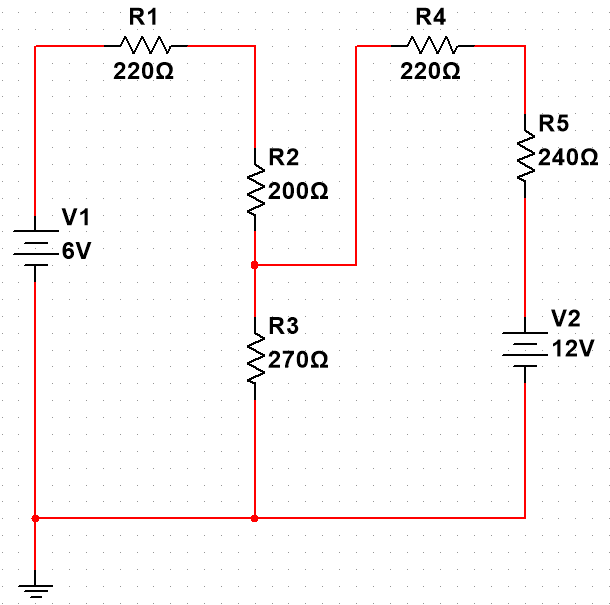
\includegraphics[width=0.4\textwidth]{ET1_3_A2-1.png}
				\caption{电路二}
				\label{fig:fig2-1}
			\end{figure}
			
			\begin{enumerate}
				\item 电路描述
				
				\begin{itemize}
					\item 电源:有两个电源,$V1$ 是 $6$ 伏特,$V2$ 是 $12$ 伏特。
					\item 电阻:有五个电阻,分别是 $R1$($220$ 欧姆)、$R2$($200$ 欧姆)、$R3$($270$ 欧姆)、$R4$($220$ 欧姆)和 $R5$($240$ 欧姆)。
				\end{itemize}
				
				\item 电路连接
				
				\begin{itemize}
					\item $R1$ 和电源 $V1$ 串联,形成电路的最左侧部分。
					\item $R4$ 和电源 $V2$ 串联,形成电路的最右侧部分。
					\item $R2$ 一端连接到 $R1$ 和 $V1$ 的连接点,另一端与 $R3$ 和 $R4$ 的连接点相连。
					\item $R3$ 一端与 $R2$ 和 $R4$ 的连接点相连,另一端直接连接到电路的负极。
					\item $R5$ 直接跨接在 $V2$ 的两端。
				\end{itemize}
				
				\item 电路工作原理分析
				
				\begin{itemize}
					\item KCL(基尔霍夫电流定律):这个电路有几个节点,在这些节点处,流入和流出的电流必须平衡。
					\item KVL(基尔霍夫电压定律):在此电路中,我们可以找到两个独立闭合回路,第一个是包含 $V1$、$R1$、$R2$ 和 $R3$ 的回路;第二个是包含 $V2$、$R4$、$R2$ 和 $R3$ 的回路。在每个闭合回路中,沿途经过的电压降之和必须等于电源电压。
					\item 叠加原理:若要用叠加原理分析这个电路,我们需要分别考虑 $V1$ 和 $V2$ 对整个电路的影响。在考虑 $V1$ 的影响时,$V2$ 被视为短路(即忽略),反之亦然。
				\end{itemize}
			\end{enumerate}
			
			这个电路可用于分析不同电阻值下电源如何共同作用于电路,以及如何使用 KCL 和 KVL 来计算复杂电路中的电流和电压分布。此外,通过改变电阻值可以观察到电流和电压如何随之改变,从而深入理解电路的工作原理。
			
			\item 电路三(如图所示)
			
			\begin{figure}[htbp]
				\centering
				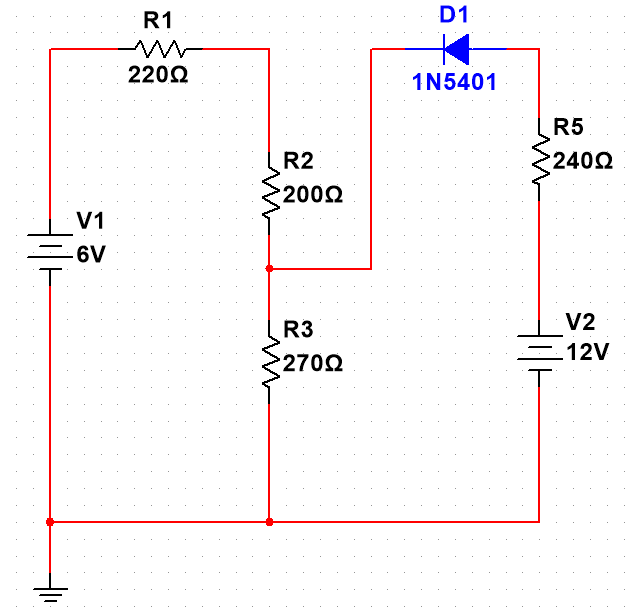
\includegraphics[width=0.4\textwidth]{ET1_3_A3-1.png}
				\caption{电路三}
				\label{fig:fig3-1}
			\end{figure}
			
			\begin{enumerate}
				\item 电路描述
				
				\begin{itemize}
					\item 电源:有两个电源,$V1$ 是 $6$ 伏特,$V2$ 是 $12$ 伏特。
					\item 电阻:电路包含四个电阻,$R1$($220$ 欧姆)、$R2$($200$ 欧姆)、$R3$($270$ 欧姆)和 $R5$($240$ 欧姆)。
					\item 二极管:电路中包含了一个二极管 $D1$(1N5401型号),这是一种标准整流二极管。
				\end{itemize}
				
				\item 电路连接
				
				\begin{itemize}
					\item $R1$ 与电源 $V1$ 串联,构成电路的左侧部分。
					\item $R5$ 与电源 $V2$ 串联,并且二极管 $D1$ 被接入 $R5$ 和 $V2$ 之间,二极管的阴极(带有标记线的一端)朝向电阻 $R5$。
					\item $R2$ 的一端与 $R1$ 和 $V1$ 的连接点相连,另一端则与 $R3$ 和 $R4$(通过二极管 $D1$)的连接点相连。
					\item $R3$ 的一端与 $R2$ 和 $R4$ 的连接点相连,另一端直接连接到电路的负极。
				\end{itemize}
				
				\item 电路工作原理分析
				
				\begin{itemize}
					\item 由于二极管的存在,电路的行为将会依赖于二极管的导电方向。当 $V2$ 的正极高于其阴极时,$D1$ 将导通,电流可以通过它流动。否则,$D1$ 将关闭,阻止电流流动。
					\item KCL(基尔霍夫电流定律):该电路具有多个节点,其中进入节点的电流必须等于离开节点的电流。
					\item KVL(基尔霍夫电压定律):在该电路中,我们可以识别两个主要的闭合回路,每个回路都包含一个电源和若干电阻,以及一个二极管。根据 KVL,沿闭合回路的电压降总和应该等于回路中电源的总电压。
				\end{itemize}
				
				\item 二极管的作用:
				
				二极管 $D1$ 会根据其正向或反向偏置的状态,影响电路中的电流流向。当 $V2$ 比 $V1$ 的电压高时,$D1$ 导通,允许电流通过。这时,$R4$ 和 $R2$、$R3$ 形成串并联组合。如果 $V2$ 的电压较低,$D1$ 会截止,这时电路中的一部分会断开。
			\end{enumerate}
			
			二极管的引入使得电路的行为比没有二极管时更复杂。需要通过实际测量或仿真来确定二极管的状态以及它对电路总体行为的影响。二极管的包含可以用来模拟例如电源切换、信号整形等情况。
			
			\item 电路四(如图所示)
			
			\begin{figure}[htbp]
				\centering
				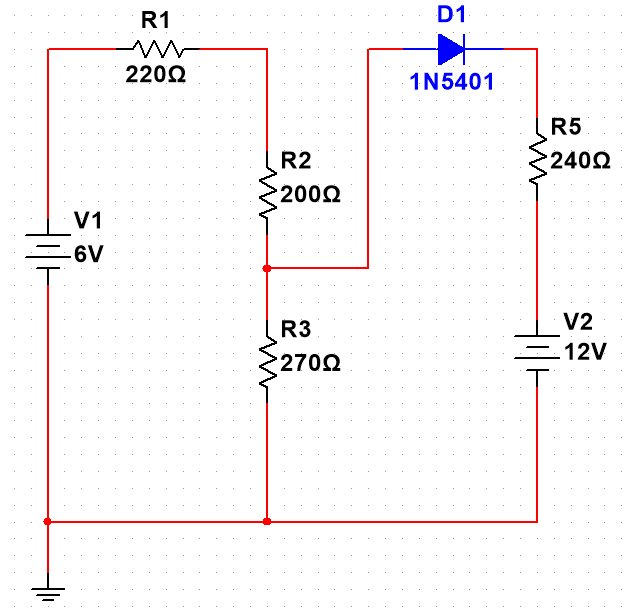
\includegraphics[width=0.4\textwidth]{ET1_3_A4-1.png}
				\caption{电路四}
				\label{fig:fig4-1}
			\end{figure}
			
			\begin{enumerate}
				\item 电路描述
				
				\begin{itemize}
					\item 电源:有两个直流电源,$V1$ 是 $6$ 伏特,$V2$ 是 $12$ 伏特。
					\item 电阻:电路包含四个电阻,它们分别是 $R1$($220$ 欧姆)、$R2$($200$ 欧姆)、$R3$($270$ 欧姆)和 $R5$($240$ 欧姆)。
					\item 二极管:电路中有一个1N5401型号的二极管 $D1$,它是一个常见的整流二极管。
				\end{itemize}
				
				\item 电路连接
				
				\begin{itemize}
					\item $R1$ 与电源 $V1$ 串联连接,构成电路的最左侧部分。
					\item $R2$ 的一端连接到 $R1$ 的另一端,另一端连接到 $R3$ 的顶部。
					\item $R3$ 连接到电路的公共地线,形成 $R2$ 和 $R3$ 的串联组合。
					\item $R5$ 与电源 $V2$ 串联连接,并且与二极管 $D1$ 串联,二极管的阴极(通常是带有标记线的一端)朝向 $R5$,构成电路的最右侧部分。
				\end{itemize}
				
				\item 电路工作原理
				
				\begin{itemize}
					\item 当 $V2$ 的正极电压高于其连接点的电压时,$D1$ 将导通,允许电流流过。这样,电路右侧的部分将由 $V2$ 供电,电流会流过 $R5$ 和 $D1$。
					\item 如果 $V2$ 的正极电压低于连接点电压,$D1$ 将截止,电流将无法通过这一部分电路。
					\item $R1$、$R2$ 和 $R3$ 的连接形式允许 $V1$ 提供电流给它们。$R2$ 和 $R3$ 形成了一个分压器,节点之间的电压取决于这两个电阻的值和它们上的电流。
				\end{itemize}
				
				\item 二极管 $D1$ 的作用
				
				\begin{itemize}
					\item 二极管的加入显著改变了电路的特性。当 $D1$ 导通时,它会影响电路右侧电压和电流的分布;当它截止时,右侧电路会从电路中断开。
					\item $D1$ 的方向决定了 $V2$ 是否能影响整个电路。当 $D1$ 导通时,$V2$ 可以对 $R2$ 和 $R3$ 施加影响,否则,它们只受 $V1$ 的影响。
				\end{itemize}
			\end{enumerate}
			
			此电路的设计可以用于模拟诸如电源选择、信号整流或电路保护等场景。通过测量和分析不同点的电压和电流,可以了解电源如何协同工作以及二极管如何控制电路的行为。
			
		\end{enumerate}
		
		\item \textbf{电路仿真}
		
		接着我们基于上述四个电路,利用软件Multisim进行了仿真,仿真结果呈列如下。
		
		\begin{enumerate}
			\item 仿真一(如图所示)
			
			\begin{figure}[htbp]
				\centering
				\subfloat[]{
					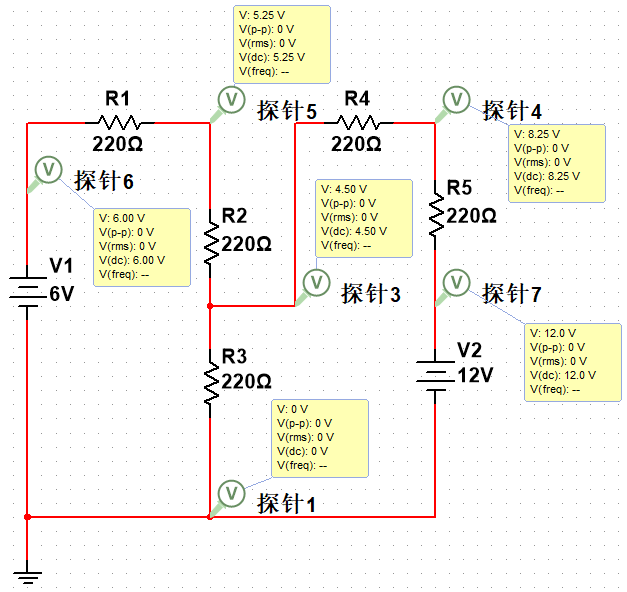
\includegraphics[width=0.4\textwidth]{ET1_3_A1-2.png}
				}
				\subfloat[]{
					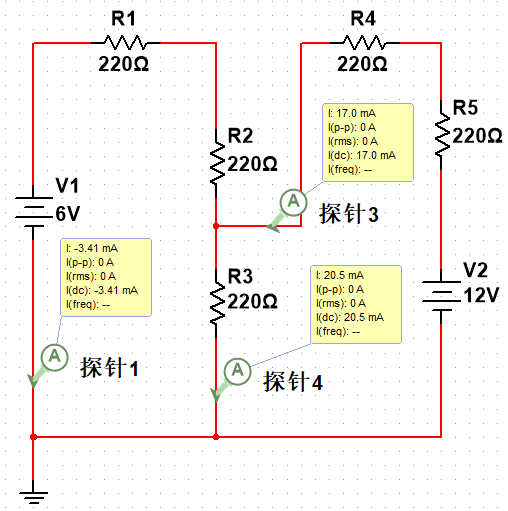
\includegraphics[width=0.4\textwidth]{ET1_3_A1-3.png}
				}
				\caption{仿真一}
				\label{fig:fig1-2}			
			\end{figure}
			
			\begin{enumerate}
				\item \textbf{电压仿真结果(根据第一张图片):}
				
				\begin{enumerate}
					\item 节点1(R3与负极连接处)的电压为 $0$ V,这是因为它直接连接到电路的公共地或参考点。
					\item 节点2(R2与R3之间)的电压为 $4.50$ V。
					\item 节点3(R2与R1、R4之间)的电压为 $4.50$ V。
					\item 节点4(R5与R4连接处)的电压为 $8.25$ V。
					\item 节点5(R1与正极 $V1$ 连接处)的电压为 $5.25$ V。
					\item 节点6(R1与R2连接处)的电压为 $6.00$ V。
					\item 节点7(R5与正极 $V2$ 连接处)的电压为 $12.00$ V。
				\end{enumerate}
				
				节点电压的分布反映了 KVL 的应用,每个回路内的电压降加起来等于电源电压。
				
				\item \textbf{电流仿真结果(根据第二张图片):}
				
				\begin{enumerate}
					\item 电流 $I1$(通过 R3 的电流)为 $20.5$ mA。
					\item 电流 $I2$(通过 R2 的电流)为 $17.0$ mA。
					\item 电流 $I3$(通过 R1 的电流)为 $34.1$ mA。
					\item 电流 $I4$(通过 R4 的电流)为 $17.0$ mA。
				\end{enumerate}
				
				电流的分布遵循了 KCL,即进入任何节点的电流等于离开节点的电流。例如,通过 R1 进入节点6的电流($34.1$ mA)分为通过 R2 离开的电流($17.0$ mA)和通过 R3 离开的电流($20.5$ mA),两者相加等于 $34.1$ mA(存在一些误差可能是由于仿真的精度或四舍五入导致)。
				
				\item \textbf{分析:}
				\begin{itemize}
					\item 通过观察节点6和节点5之间的电压差($6.00$ V - $5.25$ V = $0.75$ V),我们可以计算出 R1 上的实际电压降是 $0.75$ V,而不是整个电源电压 $6$ V。这是因为 R2 和 R3 的并联组合也分担了部分电压。
					\item 类似地,节点7和节点4之间的电压差($12.00$ V - $8.25$ V = $3.75$ V)表示 R4 上的电压降是 $3.75$ V。
					\item R5 直接跨接在电源 $V2$ 上,因此其两端电压就是 $V2$ 的电压,即 $12$ V。
					\item 电流的计算显示,电流 $I1$ 和 $I4$ 通过 R3 和 R4 时相同($17.0$ mA),这意味着在这一分支上没有其他并联分支。但是,电流 $I3$($34.1$ mA)比 $I2$($17.0$ mA)和 $I1$($20.5$ mA)都要大,表明 R1 上的电流是分流到 R2 和 R3 的。
				\end{itemize}
				
			\end{enumerate}
			
			\item 仿真二(如图所示)
			
			\begin{figure}[htbp]
				\centering
				\subfloat[]{
					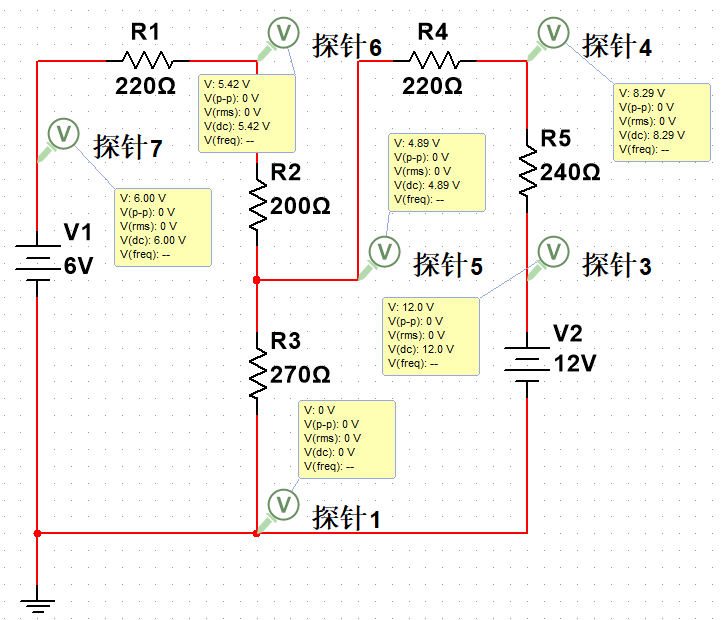
\includegraphics[width=0.4\textwidth]{ET1_3_A2-2.png}
				}
				\subfloat[]{
					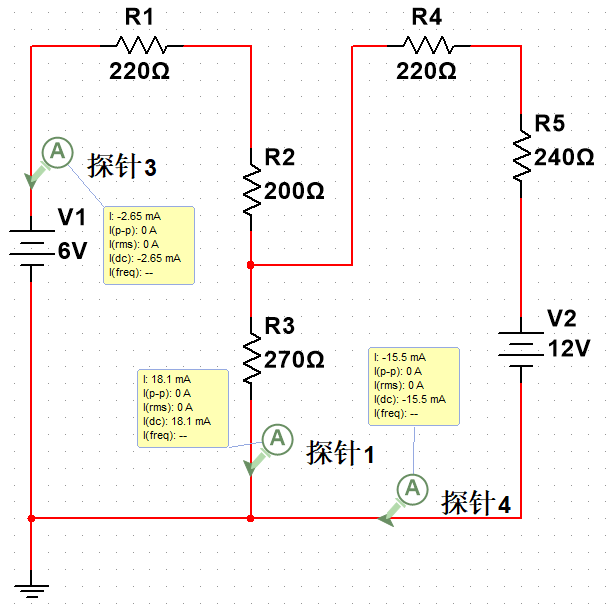
\includegraphics[width=0.4\textwidth]{ET1_3_A2-3.png}
				}
				\caption{仿真二}
				\label{fig:fig2-2}			
			\end{figure}
			
			\begin{enumerate}
				\item \textbf{电压仿真结果(根据第一张图片):}
				
				\begin{enumerate}
					\item 节点1(R3的底端)的电压为 $0$ V,这是因为它是电路的地点。
					\item 节点2(R2与R3的连接点)的电压为 $4.89$ V。
					\item 节点3(R5的顶端)的电压为 $8.29$ V。
					\item 节点4(R4的顶端)的电压为 $5.42$ V。
					\item 节点5(R2与R4的连接点)的电压为 $4.89$ V。
					\item 节点6(R1的顶端)的电压为 $6.00$ V。
					\item 节点7(R5的底端)的电压为 $12.00$ V。
				\end{enumerate}
				
				电压的读数符合 KVL,显示了电路中不同部分的电压降。注意节点6和节点7显示的是整个电源的电压,而节点2和节点3显示的是电路中间点的电压降。
				
				\item \textbf{电流仿真结果(根据第二张图片):}
				
				\begin{enumerate}
					\item 电流 $I1$(通过 R3 的电流)为 $18.1$ mA。
					\item 电流 $I2$(通过 R2 的电流)为 $15.5$ mA。
					\item 电流 $I3$(通过 R1 的电流)为 $26.5$ mA。
					\item 电流 $I4$(通过 R4 和 R5 的电流)为 $15.5$ mA。
				\end{enumerate}
				
				电流的读数遵循 KCL。在这个电路中,流入节点2的电流(通过 R1 的 $26.5$ mA)分两路流出:一路通过 R2($15.5$ mA),另一路通过 R3($18.1$ mA)。此外,电流 $I4$ 通过 R4 和 R5,说明两个电阻上的电流相同,因为它们串联在同一电源 $V2$ 上。
				
				\item \textbf{分析:}
				\begin{itemize}
					\item R1 和 R2、R3 并联,其上的电流之和等于 $26.5$ mA,这个电流是由电源 $V1$ 供给的。
					\item R4 和 R5 串联,它们上的电流相同,这是因为串联电路中电流是恒定的。
					\item 电压降分布反映了电阻的值和位置,如 R5 上的电压降($12.00$ V - $8.29$ V = $3.71$ V)较高,因为它有更高的阻值($240$ 欧姆)。
					\item 在没有外部负载的情况下,R3 上没有电压降,因为它直接连接到地点,这解释了节点1为 $0$ V 的原因。
				\end{itemize}
			\end{enumerate}
			
			\item 仿真三(如图所示)
			
			\begin{figure}[htbp]
				\centering
				\subfloat[]{
					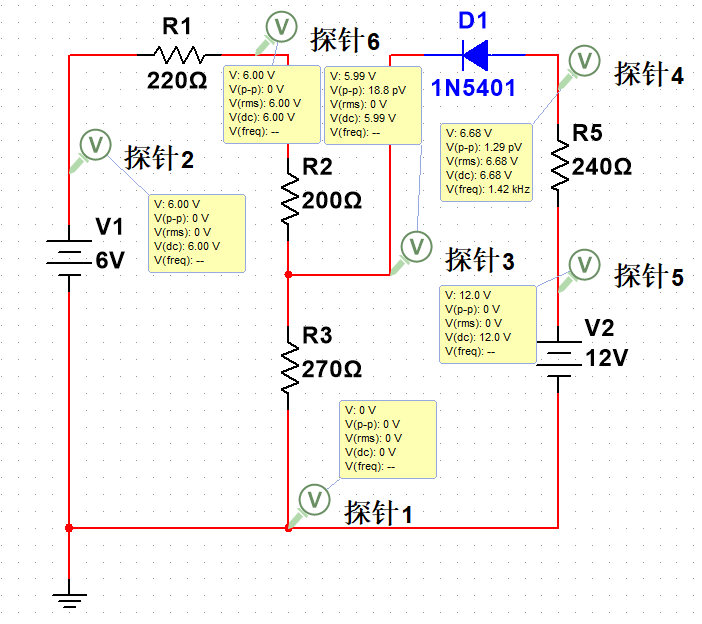
\includegraphics[width=0.4\textwidth]{ET1_3_A3-2.png}
				}
				\subfloat[]{
					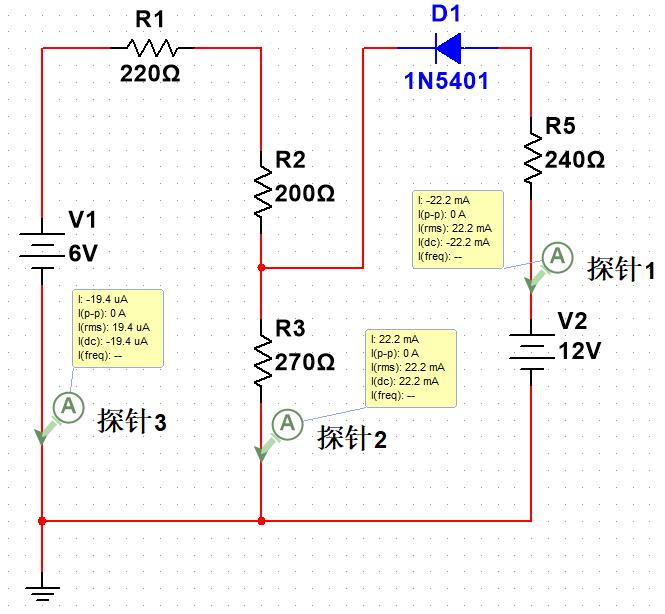
\includegraphics[width=0.4\textwidth]{ET1_3_A3-3.png}
				}
				\caption{仿真三}
				\label{fig:fig3-2}			
			\end{figure}
			
			\begin{enumerate}
				\item \textbf{电压仿真结果(根据第一张图片):}
				
				\begin{enumerate}
					\item 节点1(R3与负极相连)的电压为 $0$ V,作为电路的地点。
					\item 节点2(R2与R3连接处)的电压为 $5.99$ V。
					\item 节点3(R2与R1、D1连接处)的电压为 $6.68$ V。
					\item 节点4(R5与D1连接处)的电压为 $6.68$ V。
					\item 节点5(R5与V2连接处)的电压为 $12.0$ V。
					\item 节点6(R1与V1连接处)的电压为 $6.0$ V。
				\end{enumerate}
				
				电压结果显示,二极管 D1 的前后存在电压降,这表明二极管是导通的。节点5和节点4的电压差($12.0$ V - $6.68$ V = $5.32$ V)反映了 R5 上的电压降。节点6显示了电源 V1 的电压,这是因为节点6是 R1 的顶部和 $V1$ 的正极相连接的地方。
				
				\item \textbf{电流仿真结果(根据第二张图片):}
				
				\begin{enumerate}
					\item 电流 $I1$(通过 R5 和 D1 的电流)为 $22.2$ mA。
					\item 电流 $I2$(通过 R3 的电流)为 $22.2$ mA。
					\item 电流 $I3$(通过 R1 的电流)为 $19.4$ $\mu$A。
				\end{enumerate}
				
				这些电流读数表明,电路中的电流主要由 $V2$ 电源提供,因为 $R5$ 和 $D1$ 的电流相同,说明二极管 D1 是导通的。由于 $V1$ 电源的电压较低,它在电路中提供的电流非常小,这从 $R1$ 上的微小电流($19.4$ $\mu$A)可以看出。
				
				\item \textbf{分析:}
				\begin{itemize}
					\item 二极管 D1 导通,使得大部分电流都由 $V2$ 供应,流过 $R5$ 和 $D1$。
					\item $V1$ 电源对整个电路的贡献很小,这可能是因为 $V1$ 电源的电压小于二极管 D1 与节点3之间的电压,因此无法克服该电压降而导致流过 $R1$ 的电流几乎为零。
					\item $R2$ 和 $R3$ 上的电压降表明它们在 $V2$ 供应的电流下工作。
				\end{itemize}
			\end{enumerate}
			
			\item 仿真四(如图所示)
			
			\begin{figure}[htbp]
				\centering
				\subfloat[]{
					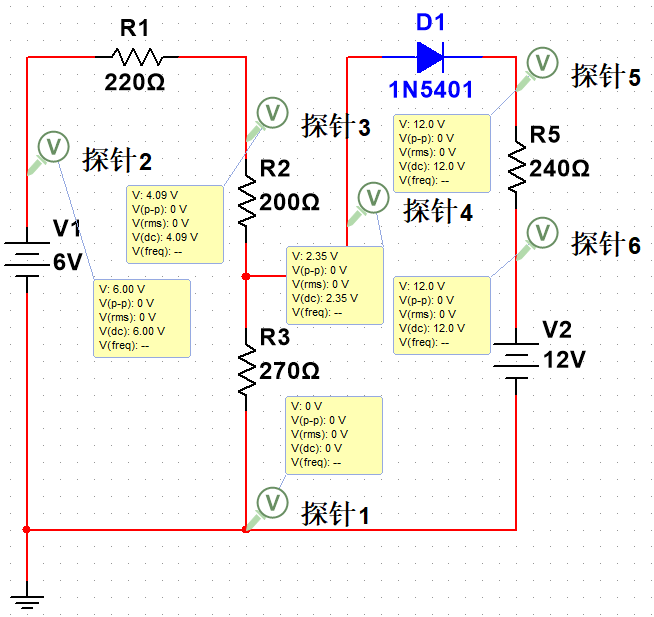
\includegraphics[width=0.4\textwidth]{ET1_3_A4-2.png}
				}
				\subfloat[]{
					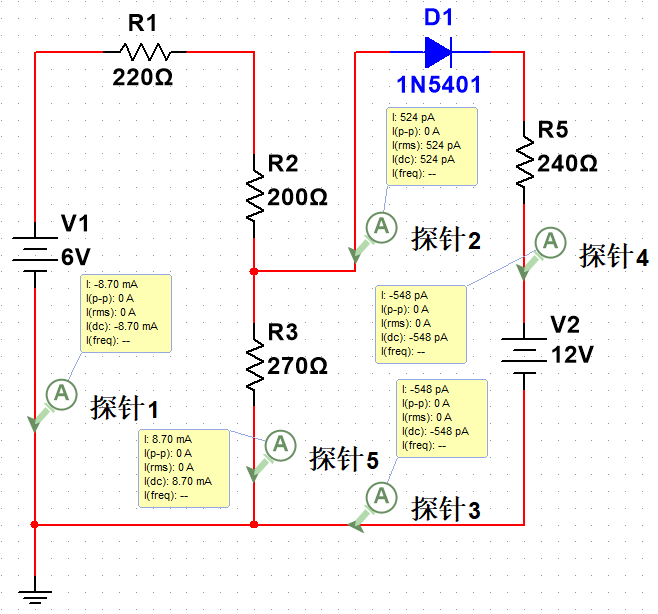
\includegraphics[width=0.4\textwidth]{ET1_3_A4-3.png}
				}
				\caption{仿真四}
				\label{fig:fig4-2}			
			\end{figure}
			
			\begin{enumerate}
				\item \textbf{电压仿真结果(根据第一张图片):}
				
				\begin{enumerate}
					\item 节点1(R3的底部和电路的负极)的电压为 $0$ V。节点2(R2和R3的连接点)的电压为 $2.35$ V。 
					\item 节点3(R2的顶部和R1、D1的连接点)的电压为 $4.09$ V。节点4(R5的顶部和D1的正向连接点)的电压为 $12.0$ V。 
					\item 节点5(R5和V2的连接点)的电压也为 $12.0$ V。节点6(R1和V1的连接点)的电压为 $6.0$ V。 
				\end{enumerate}
				
				由电压分布结果可见,二极管 D1 导通,允许从 $V2$ 至 $R5$ 的电流流动。此外, $R1$ 与 $V1$ 串联的节点6展现了整个 $6$ V 电压,表明无电压降在 $R1$ 上。节点2和节点3之间较小的电压差表明, $R2$ 上的电压降较小。
				
				\item \textbf{电流仿真结果(根据第二张图片):}
				
				\begin{enumerate}
					\item 电流 $I1$(通过 $R1$ 的电流)为 $8.70$ mA。电流 $I4$(通过 $R5$ 和 $D1$ 的电流)为 $524$ $\mu$A。
					\item 电流 $I2$(通过 $R2$ 的电流)为 $524$ $\mu$A。电流 $I3$(通过 $R3$ 的电流)为 $548$ $\mu$A。
				\end{enumerate}
				
				由电流分布结果可知, $R1$ 、 $R2$ 和 $R3$ 串联在 $V1$ 上。 $R3$ 上的电流( $548$ $\mu$A)略高于 $R2$ ( $524$ $\mu$A),可能是由于仿真精度误差或者电路内的并联分支。 $R5$ 上的电流( $524$ $\mu$A)直接来自 $V2$,表明 $V2$ 的作用是主导的。
				
				\item \textbf{分析:}
				\begin{itemize}
					\item 由于 $R5$ 串联在 $D1$ 与 $V2$ 之间,节点5与节点4间没有电压降,这表明 D1 正向偏置下的压降非常小(一般二极管正向导通压降约为 $0.7$ V),且未在仿真中显示。
					\item 而节点3显示的电压( $4.09$ V)低于 $V1$ 的电压( $6$ V),表明在 $R1$ 上有一定的电压降。
					\item $R2$ 和 $R3$ 在节点2处表现出更小的电压( $2.35$ V),这意味着 $R2$ 和 $R3$ 上存在电压降。
					\item 考虑到 $V1$ 的电压低于 $V2$,且 $V1$ 与 $V2$ 的电路部分是分开的,我们可以推断 $V1$ 对 $R2$ 和 $R3$ 的影响较小,主要电流由 $V2$ 提供。
				\end{itemize}
			\end{enumerate}
			
		\end{enumerate}
		
	\end{enumerate}
	
	% 实验前思考题
%	\subsection{实验预习题}
	
	% 思考题1
%	\begin{question}
		
%	\end{question}
	
	% 思考题2
%	\begin{question}
		
%	\end{question}
	
	% 思考题3
%	\begin{question}
		
%	\end{question}
	
	% ---
	
	
	
	% 实验记录	
	\clearpage
	
	% 顶栏
	\begin{table}
		\renewcommand\arraystretch{1.7}
		\centering
		\begin{tabularx}{\textwidth}{|X|X|X|X|}
			\hline
			专业: & 物理学 & 年级: & 2022级 \\
			\hline
			姓名: & 戴鹏辉 & 学号: & 22344016\\
			\hline
			室温: &  & 实验地点: & A522 \\
			\hline
			学生签名:& 见\textbf{附件}部分 & 评分: &\\
			\hline
			实验时间:& 2024// & 教师签名:&\\
			\hline
		\end{tabularx}
	\end{table}
	% ---
	
	% 小标题
	\section{ET1-3 基尔霍夫定律和叠加原理  \quad\heiti 实验记录}
	% ---
	
	% 实验过程记录
	\subsection{实验内容、步骤与结果}
	
	%
	\subsubsection{操作步骤记录}
	\begin{enumerate}
		\item 
	\end{enumerate}	
	
	%
	\subsubsection{}
	\begin{enumerate}
		\item \begin{table}[h]
			\centering
			\caption{表格示例}
			\label{tab:tab1}
			\begin{tabular}{|c|c|c|c|c|c|}
				\hline
				组1/序号i & 1 & 2 & 3 & 4 & 5 \\
				$v_{1i}(m/s)$ & 1.26 & 1.08 & 1.00 & 0.75 & 0.38 \\
				$f_{1i}(Hz)$ & 40073 & 40127 & 40105 & 40088 & 40066 \\
				\hline
				组2/序号i & 1 & 2 & 3 & 4 & 5 \\
				$v_{2i}(m/s)$ & 1.21 & 1.06 & 0.99 & 0.52 & 0.57 \\
				$f_{2i}(Hz)$ & 40143 & 40125 & 40084 & 40080 & 40067 \\
				\hline
				组3/序号i & 1 & 2 & 3 & 4 & 5 \\
				$v_{3i}(m/s)$ & 1.15 & 0.98 & 0.78 & 0.59 & 0.36 \\
				$f_{3i}(Hz)$ & 40135 & 40115 & 40092 & 40070 & 40044 \\
				\hline
			\end{tabular}
		\end{table}		
	\end{enumerate}
	
	% ---
	
	% 原始数据
	\clearpage
	\subsection{原始数据记录}
	实验记录本上的原始数据见%\cref{}(签字)。
	
	实验台桌面整理见%\textbf{附件}部分(\cref{})。
	
	其它原始数据见%\cref{}。
	% ---
	
	% 问题记录
	\subsection{实验过程遇到问题及解决办法}
	\begin{enumerate}
		\item 
	\end{enumerate}
	% ---
	
	
	
	% 分析与讨论	
	\clearpage
	
	% 顶栏
	\begin{table}
		\renewcommand\arraystretch{1.7}
		\begin{tabularx}{\textwidth}{|X|X|X|X|}
			\hline
			专业:& 物理学 &年级:& 2022级\\
			\hline
			姓名: & 戴鹏辉 & 学号:& 22344016\\
			\hline
			日期:& 2023/11/23 & 评分: &\\
			\hline
		\end{tabularx}
	\end{table}
	% ---
	
	% 小标题
	\section{ET1-3 基尔霍夫定律和叠加原理 \quad\heiti 分析与讨论}
	% ---
	
	% 数据处理
	\subsection{实验数据分析}
	
	%
	\subsubsection{}
	\begin{enumerate}
		\item 
	\end{enumerate}
	
	%
	\subsubsection{}
	\begin{enumerate}
		\item 
	\end{enumerate}
	
	%
	\subsubsection{}
	
	% ---
	
	% 实验后思考题
	\subsection{实验后思考题}
	
	%思考题1
	\begin{question}
		
	\end{question}
	
	% 思考题2
	\begin{question}
		
	\end{question}
	
	% 思考题3
	\begin{question}
		
	\end{question}
	
	% ---
	
	
	% 结语部分
	\clearpage
	
	% 小标题
	\section{ET1-3 基尔霍夫定律和叠加原理 \quad\heiti 结语}
	% ---
	
	% 总结、杂谈与致谢
	\subsection{实验心得和体会、意见建议等}
	\begin{enumerate}
		\item 
	\end{enumerate}
	% ---
	
	% 参考文献
	\subsection{参考文献}
	[1] 维基百科 https://zh.wikipedia.org
	
	[2] 沈韩.基础物理实验.——北京:科学出版社,2015.2 ISBN:978-7-03-043311-4
	
	% ---
	
	% 附件
	\subsection{附件及实验相关的软硬件资料等}
	试验台桌面整理如%\cref{}所示。
	
	实验报告个人签名如\cref{fig:name}。
	
	\begin{figure}[htbp]
		\centering
		
\includegraphics[width=0.7\textwidth]{name.png}
		\caption{个人签名}
		\label{fig:name}
	\end{figure}
	
	% ---
	
	相关代码已上传至Github。
	
	
	
\end{document}